\section{Grover-Rudolph State Preparation}
\label{sec:grover-rudolph}

In this section, we will describe the Grover-Rudolph state-preparation routine \cite{grover2002creating} in the context that it is used in this work.
We will also show the explicit circuit compilation strategy that we use in this work which reduces the required number of T/Toffoli gates.

The Grover-Rudolph state-preparation algorithm constructs quantum circuits that prepare states of the form given by:
\begin{equation}
    \ket{0^{\otimes \lceil \log_2{L} \rceil}} \rightarrow_{\textit{Grover-Rudolph}} \sum_{l=0}^L \sqrt{p(l)} \ket{l}
\end{equation}
where $p(l)$ is a probability distribution along the different indices ($l$) with the constraint that $\sum_l p(l) = 1$.

In the context of block-encodings, preparing such probability distributions can be used to construct the $Prepare$ oracle:
\begin{equation}
    \ket{0^{\otimes \lceil \log_2{L} \rceil}} \rightarrow_{\textit{Prepare}} \sum_{l = 0}^{L-1} \sqrt{|\alpha_l| / \lambda_{asp}} \ket{l}
\end{equation}
where the probability distribution is defined by the normalized magnitudes of the coefficients of the terms in the linear combination: $p(l) = |\alpha_l| / \lambda_{asp}$.

The Grover-Rudolph algorithm works by sequentially summing up the probability distribution to the left and right of a given index and then performing a rotation controlled based on the current index.

For example, given the coefficients $\alpha_0$, $\alpha_1$, $\alpha_2$, and $\alpha_3$, the Grover-Rudolph algorithm proceeds as follows:
\begin{enumerate}
    \item Perform a Pauli-Y rotation on the top (left-most) qubit in the register by an angle: $\theta = 2 \cos^{-1}\big( \sqrt{\alpha_0 + \alpha_1} \big)$.
    \item Perform a Pauli-Y rotation on the second qubit in the register, controlled on the first qubit being in the state $\ket{0}$ by an angle: $\theta = 2 \cos^{-1}\big( \sqrt{\frac{\alpha_0}{\alpha_0 + \alpha_1}} \big)$
    \item Perform a Pauli-Y rotation on the second qubit in the register, controlled on the first qubit being in the state $\ket{1}$ by an angle: $\theta = 2 \cos^{-1}\big( \sqrt{\frac{\alpha_2}{\alpha_2 + \alpha_3}} \big)$
\end{enumerate}

The evolution of the quantum state is described by:
\begin{equation}
    \begin{split}
        \ket{00} &\rightarrow_{\textit{(i)}} \sqrt{\alpha_0 + \alpha_1} \ket{00} + \sqrt{\alpha_2 + \alpha_3} \ket{10} \\
        &\rightarrow_{\textit{(ii)}} \sqrt{\alpha_0} \ket{00} + \sqrt{\alpha_1} \ket{01} + \sqrt{\alpha_2 + \alpha_3} \ket{10} \\
        &\rightarrow_{\textit{(iii)}} \sqrt{\alpha_0} \ket{00} + \sqrt{\alpha_1} \ket{01} + \alpha_2 \ket{10} + \alpha_3 \ket{11}
    \end{split}
\end{equation}

When the number of coefficients to prepare is greater than $4$ ($L > 4$), the same structure for the multiplexor operation can be used with the rotations placed throughout in order to reduce the number of T/Toffoli gates required.
A schematic for this circuit is given in Figure \ref{fig:grover-rudolph}. 
The upper-bound for the number of left (and right) elbows that are required using this construction is given by $\lceil L / 2 \rceil - 2$. \ws{Need to confirm this and give a more robust cost analysis than just an upper-bound. Want to do numerical estimates, but need to implement the code first.}
The number of ancillae qubits that are needed is $\lceil \log_2{L} \rceil - 2$ and the number of rotations that are required is $L - 1$ with only one of these rotations being uncontrolled.

\begin{figure}
    \centering
    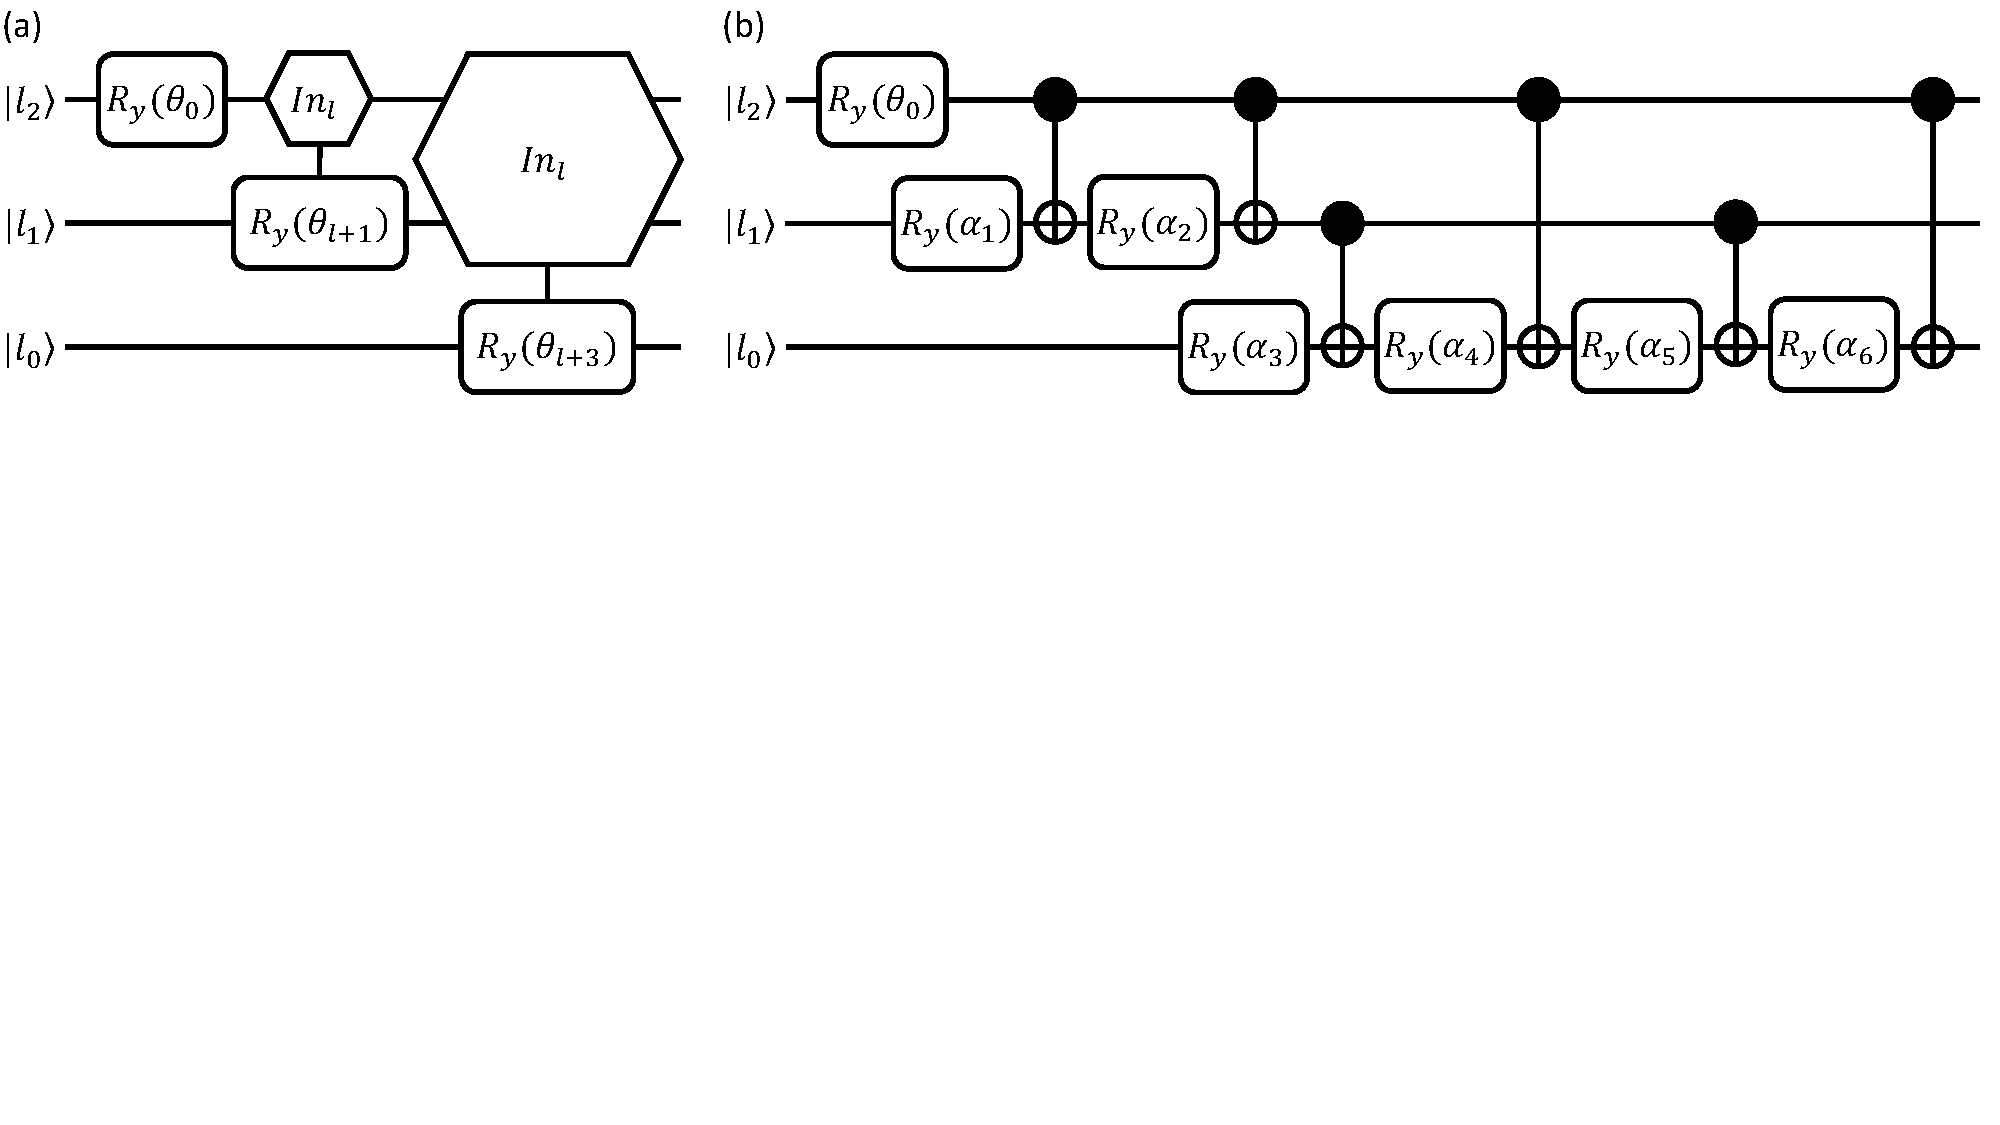
\includegraphics[width=16cm]{figures/grover-rudolph.pdf}
    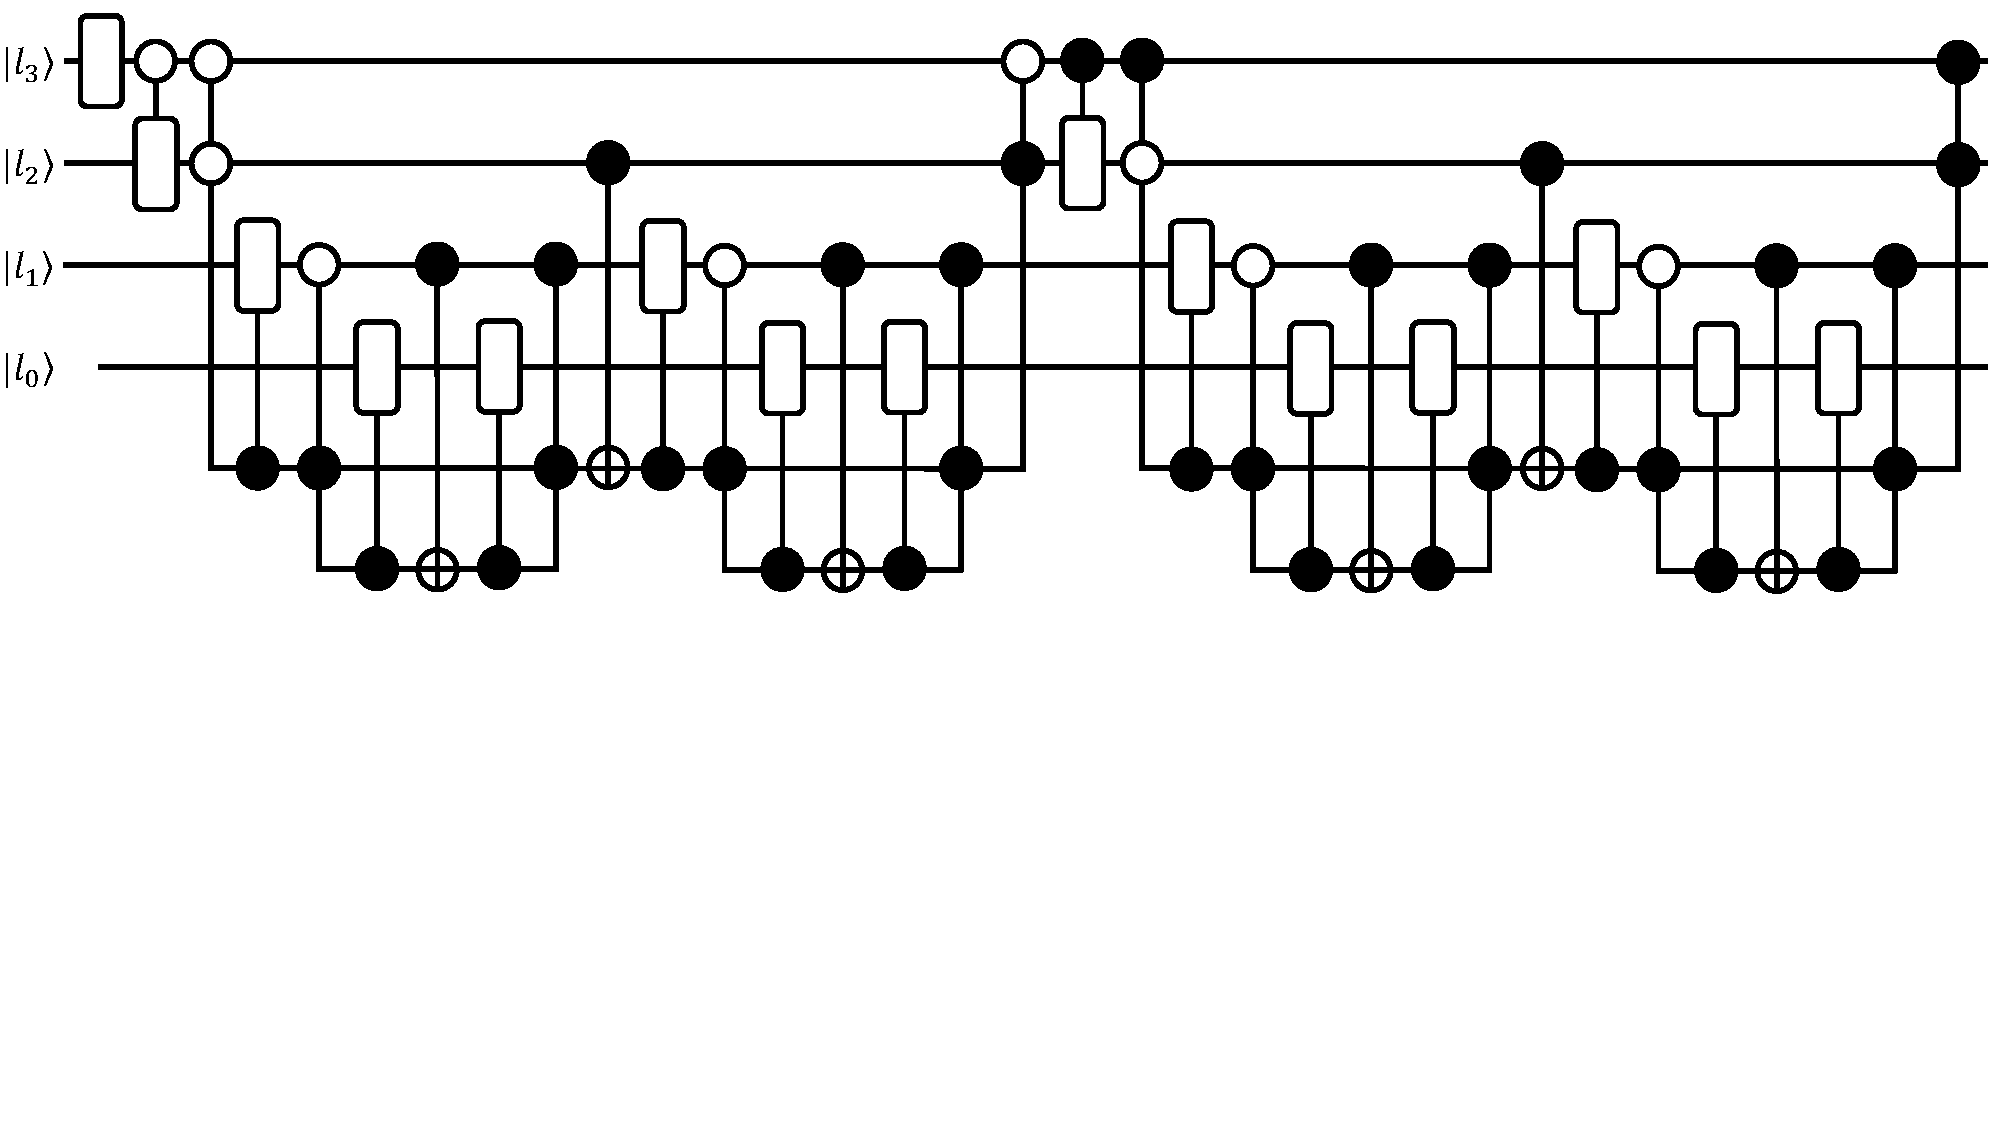
\includegraphics[width=16cm]{figures/grover-rudolph-4-qubits.pdf}
    \caption{
        \textbf{Grover-Rudolph Circuit Compilation.} 
        This figure shows an implementation of the Grover-Rudolph algorithm that leverages the same circuit structure used for multiplexing to reduce the number of T/Toffoli gates needed.
        The top subfigure shows the circuit for when 8 coefficients are being prepared.
        This circuit requires 7 rotations, 2 left (and right) elbows, and one ancilla qubit. 
        The bottom subfigure shows the structure of the circuit for when 16 coefficients are being prepared and the recursive structure of the circuit is better displayed.
        The boxes without labels represent $R_y$ rotations.
        This circuit requires 15 rotations, 6 left (and right) elbows, and two ancilla qubits.
        \ws{The 1-ctrl'd rotations on the second qubit in the middle of the circuit can be moved to the front and then the neighboring elbows should be able to be replaced by cnots.} 
    }
    \label{fig:grover-rudolph}
\end{figure}

% \begin{figure}
%     \centering
%     \includegraphics[width=8cm]{figures/grover-rudolph-numerics.pdf}
%     \caption{
%         \textbf{Numerical Gate Count Estimates of Grover-Rudolph.} 
%         This figure shows the number of left (and right) elbows required for implementing the Grover-Rudolph algorithm as outlined in Figure \ref{fig:grover-rudolph}.
%         The numerical estimates are shown in orange as a function of the number of coefficients being prepared ($L$).
%         The upper-bound of $L$ is shown in black.    
%     }
%     \label{fig:grover-rudolph-numerics}
% \end{figure}